\documentclass{report}

\input{~/dev/latex/template/preamble.tex}
\input{~/dev/latex/template/macros.tex}

\title{\Huge{}}
\author{\huge{Nathan Warner}}
\date{\huge{}}
\pagestyle{fancy}
\fancyhf{}
\lhead{Warner \thepage}
\rhead{}
% \lhead{\leftmark}
\cfoot{\thepage}
%\setborder
% \usepackage[default]{sourcecodepro}
% \usepackage[T1]{fontenc}

\begin{document}
    % \maketitle
        \begin{titlepage}
       \begin{center}
           \vspace*{1cm}
    
           \textbf{Calculus 2} \\
           Chapter 5
    
           \vspace{0.5cm}
            
                
           \vspace{1.5cm}
    
           \textbf{Nathan Warner}
    
           \vfill
                
                
           \vspace{0.8cm}
         
           
\includegraphics[width=0.4\textwidth]{~/niu/seal.png}
                
           Computer Science \\
           Northern Illinois University\\
           October 27, 2023 \\
           United States\\
           
                
       \end{center}
    \end{titlepage}
    \tableofcontents
    \pagebreak \bigbreak \noindent
    \vspace{2in} \\
    \begin{Huge}
       \textbf{Sequences and Series} 
    \end{Huge}
    \bigbreak \noindent 
    \line(1,0){490}
    \bigbreak \noindent 

    \phantomsection
    \addcontentsline{toc}{section}{5.1 Sequences}
    \section*{5.1 Sequences}
    \bigbreak \noindent 
    \phantomsection
    \addcontentsline{toc}{subsection}{Terminology of Sequences}
    \subsection*{Terminology of Sequences}
    \bigbreak \noindent 
    To work with this new topic, we need some new terms and definitions. First, an infinite sequence is an ordered list of numbers of the form
    \begin{align*}
        a_{1},\ a_{2},\ a_{3},\ ...\ a_{n},\ ....
    .\end{align*}
    \bigbreak \noindent 
    Each of the numbers in the sequence is called a term. The symbol $n$ is called the index variable for the sequence. We use the notation
    \begin{align*}
        \{a_{n}\}_{n=1}^{\infty},\ \text{or simply}\ \{a_{n}\}
    .\end{align*}
    \bigbreak \noindent 
    to denote this sequence. A similar notation is used for sets, but a sequence is an ordered list, whereas a set is not ordered. Because a particular number $a_{n}$ exists for each positive integer $n$, we can also define a sequence as a function whose domain is the set of positive integers.
     \bigbreak \noindent 
    Let’s consider the infinite, ordered list
    \begin{align*}
        2,\ 4,\ 8,\ 16,\ 32,\ ...
    .\end{align*}
    \bigbreak \noindent 
    This is a sequence in which the first, second, and third terms are given by $a_1 = 2$, $a_2 = 4$, and $a_3 = 8$. You can probably see that the terms in this sequence have the following pattern:
    \begin{align*}
        a_{1} = 2^{1},\ a_{2} = 2^{2},\ a_{3} = 2^{3},\ a_{4}= 2^{4},\ \text{and}\ a_{5} = 2^{5}
    .\end{align*}
    \bigbreak \noindent 
    Assuming this pattern continues, we can write the $n^{th}$ term in the sequence by the explicit formula $a_n = 2^{n}$. Using this notation, we can write this sequence as
    \[
    \{2n\}_{n=1}^{\infty} \quad \text{or} \quad \{2n\}.
    \]
    \bigbreak \noindent 
    Alternatively, we can describe this sequence in a different way. Since each term is twice the previous term, this sequence can be defined recursively by expressing the $n^{th}$ term $a_n$ in terms of the previous term $a_{n-1}$. In particular, we can define this sequence as the sequence $\{a_n\}$ where $a_1=2$ and for all $n \geq 2$, each term $a_n$ is defined by the \textbf{recurrence relation} $a_n = 2a_{n-1}$.

    \pagebreak \bigbreak \noindent 
    \begin{definition}[Infinite Sequence]
        An infinite sequence $\{a_n\}$ is an ordered list of numbers of the form
        \[ a_1, a_2, \ldots, a_n, \ldots \]
        The subscript $n$ is called the index variable of the sequence. Each number $a_n$ is a term of the sequence. Sometimes sequences are defined by explicit formulas, in which case $a_n = f(n)$ for some function $f(n)$ defined over the positive integers. In other cases, sequences are defined by using a recurrence relation. In a recurrence relation, one term (or more) of the sequence is given explicitly, and subsequent terms are defined in terms of earlier terms in the sequence.


    \end{definition}

    \bigbreak \noindent 
    \nt{Note that the index does not have to start at $n=1$ but could start with other integers. For example, a sequence given by the explicit formula $a_{n}=f(n)$ could start at $n=0$,in which case the sequence would be
        \begin{align*}
            a_{0},\ a_{1},\ a_{2},\ ...
        .\end{align*}
    }
    \bigbreak \noindent 
    \begin{minipage}[t]{0.52\textwidth}
        Similarly, for a sequence defined by a recurrence relation, the term $a_0$ may be given explicitly, and the terms $a_n$ for $n \geq 1$ may be defined in terms of $a_{n-1}$. Since a sequence $\{a_n\}$ has exactly one value for each positive integer $n$, it can be described as a function whose domain is the set of positive integers. As a result, it makes sense to discuss the graph of a sequence. The graph of a sequence $\{a_n\}$ consists of all points $(n, a_n)$ for all positive integers $n$. Figure 5.2 shows the graph of $\{2n\}$.
    \end{minipage}
    \begin{minipage}[t]{0.47\textwidth}
         \begin{center}
            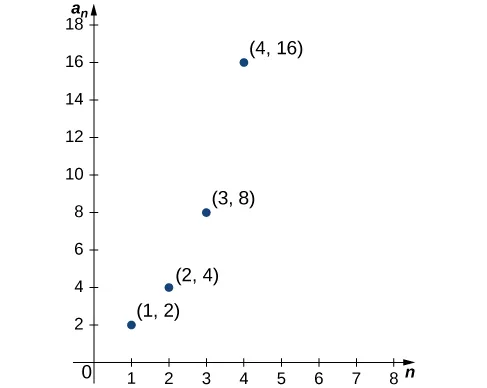
\includegraphics[scale=0.5]{./figures/mane6.png}
        \end{center}
        \begin{center}
            \textit{Figure 5.2}
        \end{center}
    \end{minipage}
    \bigbreak \noindent 
    Two types of sequences occur often and are given special names: arithmetic sequences and geometric sequences. In an arithmetic sequence, the difference between every pair of consecutive terms is the same. For example, consider the sequence
    \begin{align*}
        3,\ 7,\ 11,\ 15,\ 19,\ \cdots
    .\end{align*}
    You can see that the difference between every consecutive pair of terms is  4. Assuming that this pattern continues, this sequence is an arithmetic sequence. It can be described by using the recurrence relation
       \begin{equation}
            \begin{cases}
                a_{1} &=  3\\
                a_{n} &= a_{n-1} + 4\ \text{for } n \geq 2
            \end{cases}
        \end{equation}
    \bigbreak \noindent 
    Note that:
    \begin{align*}
        &a_{2} = 3+4 \\
        &a_{3}=  3+4+4 = 3+2\cdot 4 \\
        &a_{4} =3+4+4+4 = 3+3 \cdot 4
    .\end{align*}
    Thus the sequence can also be described using the explicit formula
    \begin{align*}
        &a_{n} = a + (n-1)d \\
        \text{Thus}\ &a_{n} = 3 + (n-1)4
    .\end{align*}
    Where $d$ is the difference $d = a_{n} - a_{n-1}$.     In general, an arithmetic sequence is any sequence of the form  $a_{n} = a +dn$
    \bigbreak \noindent 
    In a \textbf{geometric sequence}, the ratio of every pair of consecutive terms is the same. For example, consider the sequence
    \begin{align*}
        2,\ -\frac{2}{3},\ \frac{2}{9},\ -\frac{2}{27},\ \frac{2}{81},\ \cdots 
    .\end{align*}
    \bigbreak \noindent 
    We see that the ratio of any term to the preceding term is  $-\frac{1}{3}$. Assuming this pattern continues, this sequence is a geometric sequence. It can be defined recursively as
    \begin{align*}
        &a_{1} = 2 \\
        &=a_{n} = -\frac{1}{3} \cdot a_{n-1}\ \text{for } n \geq 2
    .\end{align*}
    Alternatively, since
    \begin{align*}
        &a_{2} = -\frac{1}{3} \cdot 2 \\
        &a_{3} = \left(-\frac{1}{3}\right) \left(-\frac{1}{3}\right)(2) = \left(-\frac{1}{3}\right)^{2} \cdot 2 \\
        &a_{4} = \left(-\frac{1}{3}\right)\left(-\frac{1}{3}\right)\left(-\frac{1}{3}\right) (2) = \left(-\frac{1}{3}\right)^{3} \cdot 2
    .\end{align*}
    we see that the sequence can be described by using the explicit formula
    \begin{align*}
        a_{n} = 2\left(-\frac{1}{3}\right)^{n-1}
    .\end{align*}
    The sequence \{2n\} that we discussed earlier is a geometric sequence, where the ratio of any term to the previous term is 2. In general, a geometric sequence is any sequence of the form $a_{n} = ar^{n} $.
    \pagebreak 
    \phantomsection
    \addcontentsline{toc}{subsection}{Finding explicit formulas}
    \subsection*{Finding explicit formulas}
    \bigbreak \noindent 
    \begin{eg}
       Find an explicit formula for the sequence 
       \begin{align*}
           -\frac{1}{2},\ \frac{2}{3},\ -\frac{3}{4},\ \frac{4}{5},\ -\frac{5}{6}
       .\end{align*}
    \end{eg}
    \bigbreak \noindent 
    \textbf{Solution.}
    First, note that the sequence is alternating from negative to positive. The odd terms in the sequence are negative, and the even terms are positive. Therefore, the \( n^{th} \) term includes a factor of \( (-1)^n \). Next, consider the sequence of numerators \( \{1,2,3,\ldots\} \) and the sequence of denominators \( \{2,3,4,\ldots\} \). We can see that both of these sequences are arithmetic sequences. The \( n^{th} \) term in the sequence of numerators is \( n \), and the \( n^{th} \) term in the sequence of denominators is \( n+1 \). Therefore, the sequence can be described by the explicit formula.
    \begin{align*}
        a_{n} = \frac{(-1)^{n}n}{n+1}
    .\end{align*}

    \bigbreak \noindent 
    \begin{eg}
       Find an explicit formula for the sequence
       \begin{align*}
           \frac{3}{4},\ \frac{9}{7},\ \frac{27}{10},\ \frac{81}{13},\ \frac{243}{16}
       .\end{align*}
    \end{eg}
    \bigbreak \noindent 
    \textbf{Solution.}
    The sequence of numerators \(3,9,27,81,243,\ldots\) is a geometric sequence. The numerator of the \(n^{th}\) term is \(3^n\). The sequence of denominators \(4,7,10,13,16,\ldots\) is an arithmetic sequence. The denominator of the \(n^{th}\) term is \(4+3(n-1) = 3n+1\). Therefore, we can describe the sequence by the explicit formula \(a_n = \frac{3^n}{3n+1}\).

    \bigbreak \noindent 
    \begin{eg}[Defined by Recurrence Relations]
       For each of the following recursively defined sequences, find an explicit formula for the sequence.
       \begin{enumerate}[label=(\alph*)]
           \item $a_{1} = 2,\ a_{n} = -3a_{n-1}$ for $n \geq 2 $
            \item $a_{1} = \frac{1}{2},\ a_{n} = a_{n-1} + \left(\frac{1}{2}\right)^{n} $ for $n \geq2 $
       \end{enumerate}
    \end{eg}
    \bigbreak \noindent 
    \textbf{A: Solution.} 
    \begin{align*}
        &a = 2,\ r =-3 \\
        \text{Thus:}\ &a_{n} = 2(-3)^{n-1}
    .\end{align*}
    \bigbreak \noindent 
    \textbf{B: Solution.}
    \bigbreak \noindent 
    If we write out the first few terms we get:
    \begin{align*}
        &a_{1} = \frac{1}{2},\
        a_{2} = \frac{3}{4},\
        a_{3} = \frac{7}{8},\
        a_{4} = \frac{15}{16}
    .\end{align*}
    \bigbreak \noindent 
    We see the denominator is the geometric sequence:
    \begin{align*}
        &2,\ 4,\ 8,\ 16 \\
        \text{Thus: } &a_{n} = 2^{n}
    .\end{align*}
    \bigbreak \noindent 
    And for the numerator, examining the difference between the terms, we get $2,4,8$, thus we can see that the pattern is $a_{n}  = 2^{n}-1$
    \bigbreak \noindent 
    Thus, we have the explicit formula 
    \begin{align*}
        a_{n} = \frac{2^{n}-1}{2^{n}}
    .\end{align*}

    \pagebreak 
    \phantomsection
    \addcontentsline{toc}{subsection}{Limit of a Sequence}
    \subsection*{Limit of a Sequence}
    \bigbreak \noindent 
    A fundamental question that arises regarding infinite sequences is the behavior of the terms as \( n \) gets larger. Since a sequence is a function defined on the positive integers, it makes sense to discuss the limit of the terms as \( n \to \infty \). For example, consider the following four sequences and their different behaviors as \( n \to \infty \) (see Figure 5.3):
    \begin{enumerate}
        \item $\{1+3n\} = \{4,7,10,13,\ldots\}$. The terms \(1+3n\) become arbitrarily large as \(n \to \infty\). In this case, we say that \(1+3n \to \infty\) as \(n \to \infty\).
        
        \item $\{1-\left(\frac{1}{2}\right)^{n}\} = \{\frac{1}{2},\frac{3}{4},\frac{7}{8},\frac{15}{16},\ldots\}$. The terms \(\left(1-\frac{1}{2}\right)^{n} \to 1\) as \(n \to \infty\).
        
        \item $\{(-1)^n\} = \{-1,1,-1,1,\ldots\}$.  The terms alternate but do not approach one single value as \(n \to \infty\).
        
        \item $\{\frac{(-1)^{n}}{n}\} = \{-1,\frac{1}{2},-\frac{1}{3},\frac{1}{4},\ldots\}$ 
        The terms alternate for this sequence as well, but \(\frac{(-1)^{n}}{n}  \to 0\) as \(n \to \infty\).
    \end{enumerate}
    \bigbreak \noindent 
    \begin{center}
        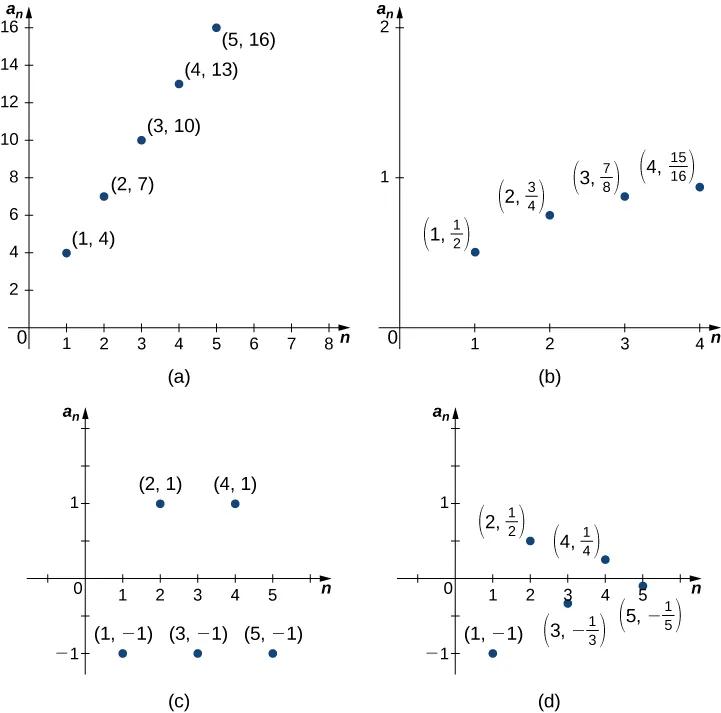
\includegraphics[scale=0.4]{./figures/mane7.png}
    \end{center}
    \bigbreak \noindent 
    From these examples, we see several possibilities for the behavior of the terms of a sequence as \( n \to \infty \). 
    In two of the sequences, the terms approach a finite number as \( n \to \infty \). 
    In the other two sequences, the terms do not. If the terms of a sequence approach a finite number \( L \) as \( n \to \infty \), 
    we say that the sequence is a convergent sequence and the real number \( L \) is the limit of the sequence. We can give an informal definition here.
    \bigbreak \noindent 
    \begin{definition}
        Given a sequence \( \{a_n\} \), \\
        if the terms \( a_n \) become arbitrarily close to a finite number \( L \) as \( n \) becomes sufficiently large, we say \( \{a_n\} \) is a convergent sequence and \( L \) is the limit of the sequence. In this case, we write \\
        \[
        \lim_{{n \to \infty}} a_n = L.
        \]
        If a sequence \( \{a_n\} \) is not convergent, we say it is a divergent sequence.
    \end{definition}

    \bigbreak \noindent 
    From Figure 5.3, we see that the terms in the sequence \( \{1-\left(\frac{1}{2}\right)^{n}\} \) are becoming arbitrarily close to 1 as \( n \) becomes very large. We conclude that \( \{1-\left(\frac{1}{2}\right)^{n}\} \) is a convergent sequence and its limit is 1. In contrast, from Figure 5.3, we see that the terms in the sequence \( 1+3n \) are not approaching a finite number as \( n \) becomes larger. We say that \( \{1+3n\} \) is a divergent sequence.
    \bigbreak \noindent 
    In the informal definition for the limit of a sequence, we used the terms “arbitrarily close” and “sufficiently large.” Although these phrases help illustrate the meaning of a converging sequence, they are somewhat vague. To be more precise, we now present the more formal definition of limit for a sequence and show these ideas graphically in Figure 5.4.
    \bigbreak \noindent 
    \begin{definition}
        A sequence \( \{a_n\} \) converges to a real number \( L \) if for all \( \varepsilon > 0 \), there exists an integer \( N \) such that \( |a_n - L| < \varepsilon \) if \( n \geq N \). The number \( L \) is the limit of the sequence and we write
        \[
        \lim_{{n \to \infty}} a_n = L \quad \text{or} \quad a_n \to L.
        \]
        In this case, we say the sequence \( \{a_n\} \) is a convergent sequence. If a sequence does not converge, it is a divergent sequence, and we say the limit does not exist.
    \end{definition}
    \bigbreak \noindent 
    We remark that the convergence or divergence of a sequence \( \{a_n\} \) depends only on what happens to the terms \( a_n \) as \( n \to \infty \). Therefore, if a finite number of terms \( b_1, b_2, \ldots, b_N \) are placed before \( a_1 \) to create a new sequence
    \[ b_1, b_2, \ldots, b_N, a_1, a_2, \ldots \]
    
    \bigbreak \noindent 
    This new sequence will converge if \( \{a_n\} \) converges and diverge if \( \{a_n\} \) diverges. Further, if the sequence \( \{a_n\} \) converges to \( L \), this new sequence will also converge to \( L \).
    \bigbreak \noindent 
    \begin{center}
        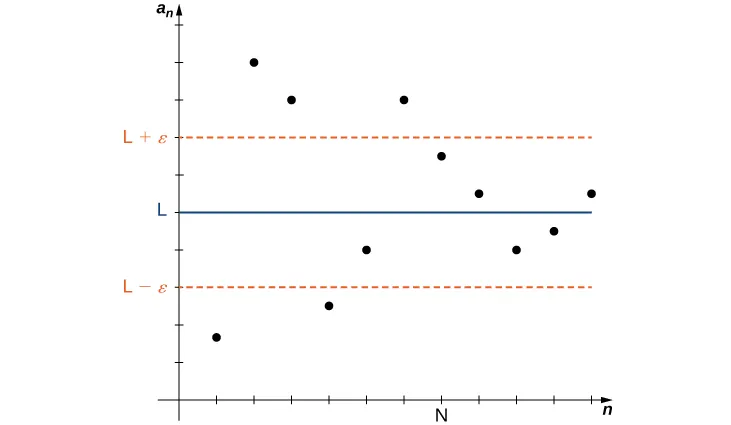
\includegraphics[scale=0.5]{./figures/mane8.png}
    \end{center}
    \bigbreak \noindent 
    As \( n \) increases, the terms \( a_n \) become closer to \( L \). For values of \( n \geq N \), the distance between each point \( (n, a_n) \) and the line \( y = L \) is less than \( \varepsilon \).
    \pagebreak \bigbreak \noindent 
    As defined above, if a sequence does not converge, it is said to be a divergent sequence. For example, the sequences \( \{1+3n\} \) and \( \{(-1)^n\} \) shown in Figure 5.4 diverge. However, different sequences can diverge in different ways. The sequence \( \{(-1)^n\} \) diverges because the terms alternate between 1 and -1, but do not approach one value as \( n \to \infty \). On the other hand, the sequence \( \{1+3n\} \) diverges because the terms \( 1+3n \to \infty \) as \( n \to \infty \). We say the sequence \( \{1+3n\} \) diverges to infinity and write
    \bigbreak \noindent 
    \[
    \lim_{{n \to \infty}} (1+3n) = \infty.
    \]
    \bigbreak \noindent 
    It is important to recognize that this notation does not imply the limit of the sequence \( \{1+3n\} \) exists. The sequence is, in fact, divergent. Writing that the limit is infinity is intended only to provide more information about why the sequence is divergent. A sequence can also diverge to negative infinity. For example, the sequence \( \{-5n+2\} \) diverges to negative infinity because \( -5n+2 \to -\infty \) as \( n \to -\infty \). We write this as
    \bigbreak \noindent 
    \[
    \lim_{{n \to \infty}} (-5n+2) = -\infty.
    \]
    \bigbreak \noindent 
    Because a sequence is a function whose domain is the set of positive integers, we can use properties of limits of functions to determine whether a sequence converges. For example, consider a sequence \( \{a_n\} \) and a related function \( f \) defined on all positive real numbers such that \( f(n) = a_n \) for all integers \( n \geq 1 \). Since the domain of the sequence is a subset of the domain of \( f \), if \( \lim_{{x \to \infty}} f(x) \) exists, then the sequence converges and has the same limit. For example, consider the sequence \( \{\frac{1}{n}\} \) and the related function \( f(x) = \frac{1}{x} \). Since the function \( f \) defined on all real numbers \( x > 0 \) satisfies \( f(x) = \frac{1}{x} \to 0 \) as \( x \to \infty \), the sequence \( \{\frac{1}{n}\} \) must satisfy \( \frac{1}{n} \to 0 \) as \( n \to \infty \).

    \bigbreak \noindent 
    \begin{thrm}[Limit of a Sequence Defined by a Function]
        Consider a sequence \( \{a_n\} \) such that \( a_n = f(n) \) for all \( n \geq 1 \). If there exists a real number \( L \) such that
        \[
        \lim_{{x \to \infty}} f(x) = L,
        \]
        then \( \{a_n\} \) converges and
        \[
        \lim_{{n \to \infty}} a_n = L.
        \]

        
    \end{thrm}

    \bigbreak \noindent 
      We now consider slightly more complicated sequences. For example, consider the sequence \( \left\{\left(\frac{2}{3}\right)^n + \left(\frac{1}{4}\right)^n\right\} \). The terms in this sequence are more complicated than other sequences we have discussed, but luckily the limit of this sequence is determined by the limits of the two sequences \( \left\{\left(\frac{2}{3}\right)^n\right\} \) and \( \left\{\left(\frac{1}{4}\right)^n\right\} \). As we describe in the following algebraic limit laws, since \( \left\{\left(\frac{2}{3}\right)^n\right\} \) and \( \left\{\left(\frac{1}{4}\right)^n\right\} \) both converge to 0, the sequence \( \left\{\left(\frac{2}{3}\right)^n + \left(\frac{1}{4}\right)^n\right\} \) converges to \( 0 + 0 = 0 \). Just as we were able to evaluate a limit involving an algebraic combination of functions \( f \) and \( g \) by looking at the limits of \( f \) and \( g \) (see Introduction to Limits), we are able to evaluate the limit of a sequence whose terms are algebraic combinations of \( a_n \) and \( b_n \) by evaluating the limits of \( \{a_n\} \) and \( \{b_n\} \).

      \bigbreak \noindent 
      \begin{thrm}[Algebraic Limit Laws]
          Given sequences \( \{a_n\} \) and \( \{b_n\} \) and any real number \( c \), if there exist constants \( A \) and \( B \) such that \( \lim_{{n \to \infty}} a_n = A \) and \( \lim_{{n \to \infty}} b_n = B \), then
          \begin{itemize}
            \item \( \lim_{{n \to \infty}} c = c \)
            \item \( \lim_{{n \to \infty}} c a_n = c \lim_{{n \to \infty}} a_n = cA \)
            \item \( \lim_{{n \to \infty}} (a_n \pm b_n) = \lim_{{n \to \infty}} a_n \pm \lim_{{n \to \infty}} b_n = A \pm B \)
            \item \( \lim_{{n \to \infty}} (a_n \cdot b_n) = (\lim_{{n \to \infty}} a_n) \cdot (\lim_{{n \to \infty}} b_n) = A \cdot B \)
            \item \( \lim_{{n \to \infty}} \frac{a_n}{b_n} = \frac{\lim_{{n \to \infty}} a_n}{\lim_{{n \to \infty}} b_n} = \frac{A}{B} \), provided \( B \neq 0 \) and each \( b_n \neq 0 \).
        \end{itemize}
      \end{thrm}

      \pagebreak \bigbreak \noindent 
      Recall that if \( f \) is a continuous function at a value \( L \), then \( f(x) \to f(L) \) as \( x \to L \). This idea applies to sequences as well. Suppose a sequence \( a_n \to L \), and a function \( f \) is continuous at \( L \). Then \( f(a_n) \to f(L) \). This property often enables us to find limits for complicated sequences. For example, consider the sequence \( \sqrt{5 - \frac{3}{n^2}} \). From Example 5.3a, we know the sequence \( 5 - \frac{3}{n^2} \to 5 \). Since \( \sqrt{x} \) is a continuous function at \( x = 5 \),
      \[ \lim_{{n \to \infty}} \sqrt{5 - \frac{3}{n^2}} = \sqrt{\lim_{{n \to \infty}} 5 - \frac{3}{n^2}} = \sqrt{5} \].
      \bigbreak \noindent 
      \begin{thrm}[Continuous Functions Defined on Convergent Sequences]
          Consider a sequence \( \{a_n\} \) and suppose there exists a real number \( L \) such that the sequence \( \{a_n\} \) converges to \( L \). Suppose \( f \) is a continuous function at \( L \). Then there exists an integer \( N \) such that \( f \) is defined at all values \( a_n \) for \( n \geq N \), and the sequence \( \{f(a_n)\} \) converges to \( f(L) \).
      \end{thrm}

      \bigbreak \noindent 
      \begin{eg}[Limits Involving Continuous Functions Defined on Convergent Sequences]
          Determine whether the sequence  $\{\cos{\left(\frac{3}{n}\right)^{2}}\} $ converges. If it converges, find its limit.
      \end{eg}
      \bigbreak \noindent 
      \textbf{Solution.} Since the sequence $\left(\frac{3}{n^{2}}\right) $ converges to 0 and $\cos{x}$ is continuous at 0, we can conclude that the sequence $\left(\frac{3}{n^{2}}\right) $ converges and
      \begin{align*}
          \lim\limits_{n \to\infty }{\cos{\left(\frac{3}{n^{2}}\right)}}= \cos{0} = 1
      .\end{align*}
      

      \bigbreak \noindent 
      Another theorem involving limits of sequences is an extension of the Squeeze Theorem for limits 
      \bigbreak \noindent 
      \begin{thrm}[Squeeze Theorem for Sequences]
          Consider sequences \( \{a_n\} \), \( \{b_n\} \), and \( \{c_n\} \). Suppose there exists an integer \( N \) such that
        \[ a_n \leq b_n \leq c_n \text{ for all } n \geq N. \]
        If there exists a real number \( L \) such that
        \[ \lim_{{n \to \infty}} a_n = L = \lim_{{n \to \infty}} c_n, \]
        then \( \{b_n\} \) converges and \( \lim_{{n \to \infty}} b_n = L \)
      \end{thrm}

      \pagebreak 
      \phantomsection
      \addcontentsline{toc}{subsection}{Bounded Sequences}
      \subsection*{Bounded Sequences}
      \bigbreak \noindent 
      We now turn our attention to one of the most important theorems involving sequences: the Monotone Convergence Theorem. Before stating the theorem, we need to introduce some terminology and motivation. We begin by defining what it means for a sequence to be bounded.

      \bigbreak \noindent 
      \begin{definition}
          A sequence \( \{a_n\} \) is bounded above if there exists a real number \( M \) such that
        \[ a_n \leq M \]
        for all positive integers \( n \).
        \bigbreak \noindent 
        A sequence \( \{a_n\} \) is bounded below if there exists a real number \( M \) such that
        \[ M \leq a_n \]
        for all positive integers \( n \).
        \bigbreak \noindent 
        A sequence \( \{a_n\} \) is a bounded sequence if it is bounded above and bounded below.
        \bigbreak \noindent 
        If a sequence is not bounded, it is an unbounded sequence.
      \end{definition}

      \bigbreak \noindent 
      For example, the sequence \( \left\{\frac{1}{n}\right\} \) is bounded above because \( \frac{1}{n} \leq 1 \) for all positive integers \( n \). It is also bounded below because \( \frac{1}{n} \geq 0 \) for all positive integers \( n \). Therefore, \( \left\{\frac{1}{n}\right\} \) is a bounded sequence. On the other hand, consider the sequence \( \{2n\} \). Because \( 2n \geq 2 \) for all \( n \geq 1 \), the sequence is bounded below. However, the sequence is not bounded above. Therefore, \( \{2n\} \) is an unbounded sequence.
      \bigbreak \noindent 
    We now discuss the relationship between boundedness and convergence. Suppose a sequence \( \{a_n\} \) is unbounded. Then it is not bounded above, or not bounded below, or both. In either case, there are terms \( a_n \) that are arbitrarily large in magnitude as \( n \) gets larger. As a result, the sequence \( \{a_n\} \) cannot converge. Therefore, being bounded is a necessary condition for a sequence to converge.

    \bigbreak \noindent 
    \begin{thrm}
        If a sequence  $\{a_{n}\} $ converges, then it is bounded. 
    \end{thrm}
    \bigbreak \noindent 
    Note that a sequence being bounded is not a sufficient condition for a sequence to converge. For example, the sequence \( \{(-1)^n\} \) is bounded, but the sequence diverges because the sequence oscillates between 1 and -1 and never approaches a finite number. We now discuss a sufficient (but not necessary) condition for a bounded sequence to converge.
    \bigbreak \noindent 
    Consider a bounded sequence \( \{a_n\} \). Suppose the sequence \( \{a_n\} \) is increasing. That is, \( a_1 \leq a_2 \leq a_3 \ldots \). Since the sequence is increasing, the terms are not oscillating. Therefore, there are two possibilities. The sequence could diverge to infinity, or it could converge. However, since the sequence is bounded, it is bounded above and the sequence cannot diverge to infinity. We conclude that \( \{a_n\} \) converges. For example, consider the sequence
    \bigbreak \noindent 
    \begin{align*}
        \bigg\{\frac{1}{2}, \frac{2}{3}, \frac{3}{4}, \frac{4}{5}, \ldots\bigg\}
    .\end{align*}
    \bigbreak \noindent 
    Since this sequence is increasing and bounded above, it converges. Next, consider the sequence

    \begin{align*}
        \{2,0,3,0,4,0,1,−\frac{1}{2},−\frac{1}{3},−\frac{1}{4},\ldots\}.
    .\end{align*}

    \bigbreak \noindent 
    \begin{definition}[]
        A sequence \( \{a_n\} \) is increasing for all \( n \geq n_0 \) if
        \[ a_n \leq a_{n+1} \text{ for all } n \geq n_0. \]
        \bigbreak \noindent 
        A sequence \( \{a_n\} \) is decreasing for all \( n \geq n_0 \) if
        \[ a_n \geq a_{n+1} \text{ for all } n \geq n_0. \]
        A sequence \( \{a_n\} \) is a \textbf{monotone sequence} for all \( n \geq n_0 \) if it is increasing for all \( n \geq n_0 \) or decreasing for all \( n \geq n_0 \).
    \end{definition}

    \bigbreak \noindent \bigbreak \noindent 
    We now have the necessary definitions to state the Monotone Convergence Theorem, which gives a sufficient condition for convergence of a sequence.
    \begin{thrm}[Monotone Convergence Theorem]
        If \( \{a_n\} \) is a bounded sequence and there exists a positive integer \( n_0 \) such that \( \{a_n\} \) is monotone for all \( n \geq n_0 \), then \( \{a_n\} \) converges.
    \end{thrm}

    % \bigbreak \noindent 
    % \begin{eg}[Monotone Convergence Theorem]
    %     Use theorem 6 to show that the sequence $\bigg\{\frac{4^{n}}{n^{!}}\bigg\} $ converges and find its limit
    % \end{eg}
    % \bigbreak \noindent 
    % Writing out the first few terms, we see that
    % \begin{align*}
    %     \bigg\{\frac{4^{n}}{n!}\bigg\} = \bigg\{4, 8, \frac{32}{3}, \frac{32}{3}, \frac{128}{15} \ldots\bigg\}. 
    % .\end{align*}
    % At first, the terms increase. However, after the third term, the terms decrease. In fact, the terms decrease for all  $n \geq 3$.
    % We can show this as follows:
    % \begin{align*}
    %     a_{n+1} = \frac{4^{n+1}}{(n+1)!} = \frac{4}{n+1} \cdot \frac{4^{n}}{n!} = \frac{4}{n+1} \cdot a_n \leq a_n \text{ if } n \geq 3.
    % .\end{align*}
    %
    % 
    % 
    % 
    %         
    %
    \bigbreak \noindent 
    \begin{eg}[Monotone Convergence Theorem]
       Determine whether the sequence is convergent or divergent. If it is convergent, find its limit. 
       \begin{align*}
           a_{n}= \frac{1000^{n}}{n!}
       .\end{align*}
    \end{eg}
    \bigbreak \noindent 
    \textbf{Solution.} 
        7.f
    \bigbreak \noindent 
    \begin{remark}
        A sequence $\{a_{n}\} $ is a monotone sequence $\forall\ n \geq n_{0}$ if it is increasing $\forall\ n \geq n_{0}$ or decreasing $\forall\ n \geq n_{0}$. If $\{a_{n}\}$ is a bounded sequence  and there exists a positive integer $n_{0}$ s.t $\{a_{n}\} $ is monotone for all $n \geq n_{0}$, then $\{a_{n}\} $ converges
    \end{remark}
    \bigbreak \noindent 
    The first thing to notice about this sequence, is that it begins by increasing, but eventually must become a decreasing sequence as $n!$ grows much faster than $1000^{n}$, to find the value of $n$ for which this switch occurs...
    \bigbreak \noindent 
    \begin{align*}
        a_{n+1} = \frac{1000^{n+1}}{(n+1)!} = \frac{1000}{n+1} \cdot  \frac{1000^{n}}{n!} = \frac{1000}{n+1}\cdot a_{n}
    .\end{align*}
    \bigbreak \noindent 
    Now that we have an equation for the $n+1$ term, we can deduce for which value of $n$ the sequence will start decreasing
    \begin{align*}
        &a_{n+1} < a_{n} \\
        & \frac{1000}{n+1} \cdot a_{n} < a_{n} \\
        &\frac{1000}{n+1} < 1 \\
        &1000 < n+1 \\
        & n > 999
    .\end{align*}
    \bigbreak \noindent 
    By induction, we can show that this is true
    \bigbreak \noindent 
    \begin{prop}
       \forall $n \geq 1000$, $a_{n} > a_{n+1} $ 
    \end{prop}
    
    \pf{Proof}{
        \bigbreak \noindent 
        \bigbreak \noindent 

        Base case: $a_{1000} > a_{1001}$ 
        \begin{align*}
               &\frac{1000^{1000}}{1000!} > \frac{1000^{1001}}{1001!}  \\
               &1000^{1000} (1001)! > 1000^{1001}(1000)! \\
               & 1000^{1000}(1001)(1000)! > 1000^{1001}(1000)! \\
               &1001 > \frac{1000^{1001}}{1000^{1000}} \\
               &10001 > 1000
        .\end{align*}
        \bigbreak \noindent 

        Inductive step: $a_{n} > a_{n+1} $ if we divide $\frac{a_{n+1}}{a_{n+2}}$ ...
        \begin{align*}
            &\frac{\frac{1000^{n}}{n!}}{\frac{1000^{n+1}}{(n+1)!}} \\
            &=\frac{1000^{n}(n+1)!}{1000^{n+1}n!} \\
            &= \frac{1000^{n}(n+1)n!}{1000^{n+1}n!} \\
            &=\frac{1000^{n}(n+1)}{1000^{n+1}} \\
            &= \frac{1}{1000}(n+1)
            % &\frac{1000^{n}}{n!} > \frac{1000^{n+1}}{(n+1)!} \\
            % &1000^{n}(n+1)! > 1000^{n+1}n! \\
            % &1000^{n}(n+1)n! > 1000^{n+1}n! \\
            % &1000^{n}(n+1) > 1000^{n+1} \\
            % &n+1 > \frac{1000^{n+1}}{1000} \\
            % &n+1 > n \quad \text{(By the fact that $\frac{x^{n}}{x^{m}} = x^{n-m}$)}
        .\end{align*}
        for $n \geq 1000 $, $\frac{1}{1000}(n+1) > 1$. $\therefore \frac{a_{n}}{a_{n+1}} > 1 \implies a_{n} > a_{n+1}$
        \bigbreak \noindent 
        
        Induction: $a_{n+1} > a_{n+2}$, we can divide $\frac{a_{n+1}}{a_{n+2}}$ 
        \begin{align*}
            &\frac{\frac{1000^{n+1}}{(n+1)!}}{\frac{1000^{n+2}}{(n+2)!}}    \\
            &= \frac{1000^{n+1}(n+2)!}{1000^{n+2}(n+1)!} \\
            &=\frac{1000^{n+1}(n+2)(n+1)!}{1000^{n+2}(n+1)!} \\
            &=\frac{1000^{n+1}(n+2)}{1000^{n+2}} \\
            &(n+2)\left(\frac{1}{1000}\right)
        .\end{align*}


        For $n \geq 1000$, $(n+2)\left(\frac{1}{1000}\right)  > 1$. $\therefore \frac{a_{n+1}}{a_{n+2}} > 1 \implies a_{n+1} > a_{n+2}$
        \bigbreak \noindent 
        \blacksquare
    }
    \bigbreak \noindent 
    Thus, this sequence is decreasing for $n \geq 1000$. Furthermore, this sequence is bounded below by $0$ because $\frac{(1000)^{n}}{n!} \geq 0,\  \forall\ n \in \mathbb{Z^{+}}$. Therefore, the conditions for the monotone convergence theorem are met and this sequence must converge.
    \bigbreak \noindent 
    Using the fact that this sequence converges, and a finite number of terms does not affect the convergence of a sequence, we can propose
    \begin{align*}
        &\lim\limits_{n \to +\infty}{a_{n+1}} = \lim\limits_{n \to +\infty}{a_{n}} = L  \\
    .\end{align*}
    \bigbreak \noindent 
    Since we know...
    \begin{align*}
        a_{n+1} = \frac{1000}{n+1}\cdot a_{n} 
    .\end{align*}
    We can take the limit of both sides, 
    \begin{align*}
        &\lim\limits_{n \to +\infty}{a_{n+1}} = \lim\limits_{n \to +\infty}{\frac{1000}{n+1}a_{n}} \\
        &L = \frac{1000}{\lim\limits_{n \to +\infty}{n+1}}\cdot \lim\limits_{n \to +\infty}{a_{n}} \\
        &L = 0 \cdot \lim\limits_{n \to +\infty}{a_{n}} \\
        &L = 0
    .\end{align*}

    \pagebreak 
    \phantomsection
    \addcontentsline{toc}{section}{5.2 Infinite Series}
    \section*{5.2 Infinite Series}
    \bigbreak \noindent 

    \begin{definition}
       An infinite series is an expression of the form
\[
\sum_{n=1}^{\infty} a_n = a_1 + a_2 + a_3 + \cdots.
\]
For each positive integer $k$, the sum
\[
S_k = \sum_{n=1}^{k} a_n = a_1 + a_2 + a_3 + \cdots + a_k
\]
is called the $k^{\text{th}}$ partial sum of the infinite series. The partial sums form a sequence $\{S_k\}$. If the sequence of partial sums converges to a real number $S$, the infinite series converges. If we can describe the convergence of a series to $S$, we call $S$ the sum of the series, and we write
\[
\sum_{n=1}^{\infty} a_n = S.
\]
If the sequence of partial sums diverges, we have the divergence of a series.
    \end{definition}
    \bigbreak \noindent 
    Note that the index for a series need not begin with $n=1$ but can begin with any value. For example, the series
    \begin{align*}
        \summation{\infty}{n=1}\ \left(\frac{1}{2}\right)^{n-1}\ 
    .\end{align*}
    Can also be written as:
    \begin{align*}
        \summation{\infty}{n=0}\ \left(\frac{1}{2}\right)^{n}\ \quad \text{or: } \summation{\infty}{n=5}\ \left(\frac{1}{2}\right)^{n-5}\  
    .\end{align*}
    \bigbreak \noindent 
    Often it is convenient for the index to begin at  1,
  so if for some reason it begins at a different value, we can reindex by making a change of variables. For example, consider the series
  \begin{align*}
      \summation{\infty}{n=2}\ \frac{1}{n^{2}}\ 
  .\end{align*}
  By introducing the variable  $m=n-1$ so that  $n=m+1$,
  we can rewrite the series as
  \begin{align*}
      \summation{\infty}{m}\ \frac{1}{(m+1)^{2}}\ 
  .\end{align*}

  \pagebreak \bigbreak \noindent 
  \begin{eg}[Evaluating Limits of Sequences of Partial Sums]
     use the sequence of partial sums to determine whether the series converges or diverges.
     \begin{align*}
         \summation{\infty}{n=1}\ \frac{n}{n+1}\ 
     .\end{align*}
  \end{eg}
  \bigbreak \noindent 
    \textbf{Solution.}
  The sequence of partial sums \( S_k \) satisfies
    \begin{align*}
        S_1 & = \frac{1}{2} \\
        S_2 & = \frac{1}{2} + \frac{2}{3} \\
        S_3 & = \frac{1}{2} + \frac{2}{3} + \frac{3}{4} \\
        S_4 & = \frac{1}{2}+ \frac{2}{3} + \frac{3}{4}+ \frac{4}{5}
    \end{align*}
    Notice that each term added is greater than  $\frac{1}{2} $ As a result, we see that
    \begin{align*}
        S_1 & = \frac{1}{2} \\
        S_2 & = \frac{1}{2} + \frac{2}{3} > \frac{1}{2} + \frac{1}{2} = 2 \left( \frac{1}{2} \right) \\
        S_3 & = \frac{1}{2} + \frac{2}{3} + \frac{3}{4} > \frac{1}{2} + \frac{1}{2} + \frac{1}{2} = 3 \left( \frac{1}{2} \right) \\
        S_4 & = \frac{1}{2} + \frac{2}{3} + \frac{3}{4} + \frac{4}{5} > \frac{1}{2} + \frac{1}{2} + \frac{1}{2} + \frac{1}{2} = 4 \left( \frac{1}{2} \right).
    \end{align*}
    From this pattern, we can see that \( S_k > k \left( \frac{1}{2} \right) \) for every integer \( k \). Therefore, \( \{ S_k \} \) is unbounded and consequently, diverges. Therefore, the infinite series 
    \[
    \sum_{n=1}^{\infty} \frac{n}{n+1}
    \]
    diverges.

    \bigbreak \noindent 
    \begin{eg}
     determine whether the series converges or diverges. 
       \begin{align*}
           \summation{\infty}{n=1}\ (-1)^{n}\ 
       .\end{align*}
    \end{eg}
    \bigbreak \noindent 
    \textbf{Solution.}
    The sequence of partial sums \( S_k \) satisfies
    \begin{align*}
        S_1 & = -1 \\
        S_2 & = -1 + 1 = 0 \\
        S_3 & = -1 + 1 - 1 = -1 \\
        S_4 & = -1 + 1 - 1 + 1 = 0.
    \end{align*}
    From this pattern, we can see the sequence of partial sums is
    \[ \{ S_k \} = \{-1, 0, -1, 0, \ldots\}. \]

    Since this sequence diverges, the infinite series 
    \[ \sum_{n=1}^{\infty} (-1)^n \]
    diverges.

    \bigbreak \noindent 
    \begin{eg}
     Determine whether the series converges or diverges. 
     \begin{align*}
         \summation{\infty}{n=1}\ \frac{1}{n(n+1)}\ 
     .\end{align*}

    \end{eg}
    \bigbreak \noindent 
    \textbf{Solution.}
    The sequence of partial sums \( S_k \) satisfies
    \begin{align*}
        S_1 & = \frac{1}{1 \cdot 2} = \frac{1}{2} \\
        S_2 & = \frac{1}{1 \cdot 2} + \frac{1}{2 \cdot 3} = \frac{1}{2} + \frac{1}{6} = \frac{2}{3} \\
        S_3 & = \frac{1}{1 \cdot 2} + \frac{1}{2 \cdot 3} + \frac{1}{3 \cdot 4} = \frac{1}{2} + \frac{1}{6} + \frac{1}{12} = \frac{3}{4} \\
        S_4 & = \frac{1}{1 \cdot 2} + \frac{1}{2 \cdot 3} + \frac{1}{3 \cdot 4} + \frac{1}{4 \cdot 5} = \frac{4}{5} \\
        S_5 & = \frac{1}{1 \cdot 2} + \frac{1}{2 \cdot 3} + \frac{1}{3 \cdot 4} + \frac{1}{4 \cdot 5} + \frac{1}{5 \cdot 6} = \frac{5}{6}.
    \end{align*}
    \bigbreak \noindent 
    From this pattern, we can see that the  $k^{th}$ partial sum is given by the explicit formula
    \begin{align*}
        S_{k} = \frac{k}{k+1}
    .\end{align*}
    \bigbreak \noindent 
    And since
    \begin{align*}
        \lim\limits_{k \to +\infty}{\frac{k}{k+1}} = 1
    .\end{align*}
    \bigbreak \noindent 
    We can conclude that the series converges, Thus:
    \begin{align*}
        \summation{\infty}{n=1}\ \frac{1}{n(n+1)}\  = 1
    .\end{align*}

    \pagebreak 
    \phantomsection
    \addcontentsline{toc}{subsection}{The Harmonic Series}
    \subsection*{The Harmonic Series}
    \bigbreak \noindent 
    A useful series to know about is the harmonic series. The harmonic series is defined as
    \begin{align*}
        \summation{\infty}{n=1}\ \frac{1}{n}  = \frac{1} + \frac{1}{2} + \frac{1}{3} + \frac{1}{4} + \ldots\ 
    .\end{align*}
    This series is interesting because it diverges, but it diverges very slowly. By this, we mean that the terms in the sequence of partial sums \( S_k \) approach infinity, but do so very slowly. We will show that the series diverges, but first, we illustrate the slow growth of the terms in the sequence \( S_k \) in the following table.
    \bigbreak \noindent 
    \begin{center}
    \begin{tabular}{|c|c|c|c|c|c|c|}
        \hline
        $k$ & $10$ & $100$ & $1,000$ & $10,000$ & $100,000$ & $1,000,000$ \\
        \hline
        $S_k$ & $2.92897$ & $5.18738$ & $7.48547$ & $9.78761$ & $12.09015$ & $14.39273$ \\
        \hline
    \end{tabular}
    \end{center}
    \bigbreak \noindent 
    Even after 1,000,000 terms, the partial sum is still relatively small. From this table, it is not clear that this series actually diverges. However, we can show analytically that the sequence of partial sums diverges, and therefore the series diverges.
    \bigbreak \noindent 
    To show that the sequence of partial sums diverges, we show that the sequence of partial sums is unbounded. We begin by writing the first several partial sums:
    \bigbreak \noindent 
    \begin{align*}
        S_1 & = 1 \\
        S_2 & = 1 + \frac{1}{2} \\
        S_3 & = 1 + \frac{1}{2} + \frac{1}{3} \\
        S_4 & = 1 + \frac{1}{2} + \frac{1}{3} + \frac{1}{4}.
    \end{align*}
    Notice that for the last two terms in \( S_4 \),
    \[
    \frac{1}{3} + \frac{1}{4} > \frac{1}{4} + \frac{1}{4}.
    \]
    Therefore, we conclude that
    \[
    S_4 > 1 + \frac{1}{2} + \left( \frac{1}{4} + \frac{1}{4} \right) = 1 + \frac{1}{2} + \frac{1}{2} = 1 + 2 \left( \frac{1}{2} \right).
    \]
    Using the same idea for \( S_8 \), we see that
    \begin{align*}
        S_8 &= 1 + \frac{1}{2} + \frac{1}{3} + \frac{1}{4} + \frac{1}{5} + \frac{1}{6} + \frac{1}{7} + \frac{1}{8} > 1 + \frac{1}{2} + \left( \frac{1}{4} + \frac{1}{4} \right) + \left( \frac{1}{8} + \frac{1}{8} + \frac{1}{8} + \frac{1}{8} \right) \\
       &= 1 + \frac{1}{2} + \frac{1}{2} + \frac{1}{2} = 1 + 3 \left( \frac{1}{2} \right)
    .\end{align*}
    \bigbreak \noindent 
    From this pattern, we see that 
    \begin{align*}
    S_1 & = 1, \\
    S_2 & = 1 + \frac{1}{2}, \\
    S_4 & > 1 + 2 \left( \frac{1}{2} \right), \\
    S_8 & > 1 + 3 \left( \frac{1}{2} \right).
    \end{align*}
    More generally, it can be shown that 
    \[ S_{2^{j}} > 1 + j \left( \frac{1}{2} \right) \]
    for all \( j > 1 \). 
    Since \( 1 + j \left( \frac{1}{2} \right) \to \infty \), we conclude that the sequence \( \{ S_k \} \) is unbounded and therefore diverges. In the previous section, we stated that convergent sequences are bounded. Consequently, since \( \{ S_k \} \) is unbounded, it diverges. Thus, the harmonic series diverges.

    \pagebreak 
    \phantomsection
    \addcontentsline{toc}{subsection}{Algebraic Properties of Convergent Series}
    \subsection*{Algebraic Properties of Convergent Series}
    \bigbreak \noindent 
    Since the sum of a convergent infinite series is defined as a limit of a sequence, the algebraic properties for series listed below follow directly from the algebraic properties for sequences.
    \bigbreak \noindent 
    \begin{thrm}[Algebraic Properties of Convergent Series]
        Let $ \sum_{n=1}^{\infty} a_n$ and $\sum_{n=1}^{\infty} b_n$ be convergent series. Then the following algebraic properties hold:
        \begin{enumerate}
            \item The series 
            $\sum_{n=1}^{\infty} (a_n + b_n)$ converges and 
            \begin{align*}
                \sum_{n=1}^{\infty} (a_n + b_n) = \sum_{n=1}^{\infty} a_n + \sum_{n=1}^{\infty} b_n. \quad \text{(Sum Rule)}
            .\end{align*}
            \item The series $\sum_{n=1}^{\infty} (a_n - b_n)$ converges and 
                \begin{align*}
                    \sum_{n=1}^{\infty} (a_n - b_n) = \sum_{n=1}^{\infty} a_n - \sum_{n=1}^{\infty} b_n. \quad \text{(Difference Rule)}
                .\end{align*}
            \item For any real number \( c \), the series $\sum_{n=1}^{\infty} c a_n$ converges and 
                \begin{align*}
                    \sum_{n=1}^{\infty} c a_n = c \sum_{n=1}^{\infty} a_n. \quad \text{(Constant Multiple Rule)}
                .\end{align*}
        \end{enumerate}
    \end{thrm}

    \bigbreak \noindent 
    \phantomsection
    \addcontentsline{toc}{subsection}{Geometric Series}
    \subsection*{Geometric Series}
    \bigbreak \noindent
    A geometric series is of the form:
    \begin{align*}
        \summation{\infty}{n=1}\ a(r)^{n-1}\  = a + ar + ar^{2} + ar^{3} + ... 
    .\end{align*}
    \bigbreak \noindent 
    So when does it converge? When $a>0$, its sequence of partial sums is given by:
    \begin{align*}
        \summation{\infty}{n=1}\ ar^{n-1}\  = a + ar + ar^{3} + ... + ar^{k-1}
    .\end{align*}
    \bigbreak \noindent 
    When $r=1$, we have:
    \begin{align*}
        S_{k} =  a + a(1) + a(1)^{2} + a(1)^{3}  +... + a(1)^{k-1}\  = ak
    .\end{align*}
    \bigbreak \noindent 
    Since $a>0$, we know that $ak \to \infty$ as $k \to \infty$, Thus, the sequence of partial sums is unbounded and diverges, which means when $r=1$ the series diverges. When $r \ne 1$, we have:
    \begin{align*}
        S_{k} = a + ar + ar^{2} + ar^{3} + ... + ar^{k-1}
    .\end{align*}
    \bigbreak \noindent 
    We can then multiply by $(1-r)$ to get some nice cancellations:
    \begin{align*}
        &(1-r)S_{k} = (1-r)(a + ar + ar^{2} + ar^{3} +... + ar^{k-1}) \\
        &(1-r)S_{k} = a(1-r)(1 + r + r^{2} + r^{3} + ... +r^{k-1}) \\
        &(1-r)S_{k} = a(1 + r -r + r^{2} - r^{2} + r^{3} - r^{3} - r^{k}) \\
        &(1-r)S_{k} = a(1-r^{k}) \\
        &S_{k} = \frac{a(1-r^{k})}{1-r} \quad \text{for $r\ne 1$}
    .\end{align*}
    \bigbreak \noindent 
    Since we know for any $r \in \mathbb{R}$, s.t $0 \leq r < 1$, $r^{k} \to 0$. Whereas $r^{k} \to \infty$ for $r>1 $. Thus, $r^{k} \to 0$ if $\abs{r} < 1$ and $r \to \infty$ if $\abs{r} > 1$. This means we can write:
    \begin{definition}
        Geometric series convergence or divergence: 
    \begin{align*}
       \summation{\infty}{n=1}\ ar^{n-1} \  = \quad \quad 
                \begin{cases}
                     \frac{a}{1-r} & \text{if }  \abs{r} < 1\\
                     diverges & \text{if }  \abs{r} \geq 1
                \end{cases}
    .\end{align*}
    \end{definition}
    \bigbreak \noindent 
    \begin{eg}
        Determine if the series converges or diverges
        \begin{align*}
            \summation{\infty}{n=1}\ \frac{(-3)^{n+1}}{4^{n-1}} \ 
        .\end{align*}
    \end{eg}
    \bigbreak \noindent 
    \textbf{Solution.} We can rewrite this as:
    \begin{align*}
        &\summation{\infty}{n=1}\ \frac{(-3)^{n-1}(-3)^{2}}{4^{n-1}}\  \\
        &=\summation{\infty}{n=1}\ 9 \left(-\frac{3}{4}\right)^{n-1}\ 
    .\end{align*}
    \bigbreak \noindent 
    Which means we have $a=9$, $r = -\frac{3}{4} $. Since $\abs{r} < 1$, this sequence converges to...
    \begin{align*}
       &\frac{a}{1-r} = \frac{9}{1+\frac{3}{4}}  \\ 
       &=9+\frac{7}{4} \\
       &=\frac{36}{7}
    .\end{align*}
    \bigbreak \noindent 
    \begin{eg}
        Determine if the series converges or diverges
        \begin{align*}
            &\summation{\infty}{n=1}\ e^{2n}\ 
        .\end{align*}
    \end{eg}
    \bigbreak \noindent 
    \textbf{Solution.} We can rewrite this as 
    \begin{align*}
        &\summation{\infty}{n=1}\ (e^{n})^{2}\  \\
        &=\summation{\infty}{n=1}\ (e^{n-1})^{2}e^{2}\  \\
        &=\summation{\infty}{n=1}\ (e^{2})^{n-1}e^{2}\ 
    .\end{align*}
    \bigbreak \noindent 
    Which means we have $r=e^{2}$. Since $\abs{r} > 1$, this series diverges

    \pagebreak \bigbreak \noindent 
    We now turn our attention to a nice application of geometric series. We show how they can be used to write repeating decimals as fractions of integers.
    \bigbreak \noindent 
    \begin{eg}[Writing Repeating Decimals as Fractions of Integers]
        Use a geometric series to write  $3.\bar{26}$ as a fraction of integers.
    \end{eg}
    \bigbreak \noindent 
    \textbf{Solution.} Since $3.\bar{26}$ = $3.262626...$, first we write 
    \begin{align*}
        &3.262626 = 3 + \frac{26}{100} + \frac{26}{10,000} + \frac{26}{1,000,000} + ...  \\
        &= 3+ \frac{26}{10^{2}} + \frac{26}{10^{4}} + \frac{26}{10^{6}} + ... 
    .\end{align*}
    \bigbreak \noindent 
    Ignoring the first term $3$, the rest of this expression is a geometric series with initial term $a = \frac{26}{10^{2}} $ and $r=\frac{1}{10^{2}} $. Thus, the sum of the series is
    \begin{align*}
        &\frac{\frac{26}{10^{2}}}{1-\left(\frac{1}{10^{2}}\right)} \\
        &=\frac{\frac{26}{10^{2}}}{\frac{99}{10^{2}}} \\
        &=\frac{26}{99}
    .\end{align*}
    \bigbreak \noindent 
    Thus $3.\bar{26}$ = 
    \begin{align*}
        &3 + \frac{26}{99} \\
        &=\frac{323}{99}
    .\end{align*}

    \pagebreak \bigbreak \noindent 
    \phantomsection
    \addcontentsline{toc}{section}{5.3 The Divergence and Integral Tests}
    \section*{5.3 The Divergence and Integral Tests}
    \bigbreak \noindent 
    \phantomsection
    \addcontentsline{toc}{subsection}{Divergence Test}
    \subsection*{Divergence Test}
    \bigbreak \noindent 
    For a series $\sum_{n=1}^{\infty} a_n$ to converge, the $n$th term $a_n$ must satisfy $a_n \to 0$ as $n \to \infty$.
    \bigbreak \noindent 
    Therefore, from the algebraic limit properties of sequences,
    \[
    \lim_{k \to \infty} a_k = \lim_{k \to \infty} (S_k - S_{k-1}) = \lim_{k \to \infty} S_k - \lim_{k \to \infty} S_{k-1} = S - S = 0.
    \]
    Therefore, if $\sum_{n=1}^{\infty} a_n$ converges, the $n$th term $a_n \to 0$ as $n \to \infty$. An important consequence of this fact is the following statement:
    \begin{align*}
        \text{If } a_n \nrightarrow 0\ \text{as } n \to \infty, \sum_{n=1}^{\infty} a_n\ \text{diverges.}
    .\end{align*}
    \bigbreak \noindent 
    This test is known as the divergence test because it provides a way of proving that a series diverges.
    \bigbreak \noindent 
    \begin{thrm}[Divergence Test]
        In the context of sequences, if $\lim_{{n \to \infty}} a_n = c \neq 0$ or the limit does not exist, then the series $\sum_{{n=1}}^{\infty} a_n$ is said to diverge.
    \end{thrm}
    \bigbreak \noindent 
    It is important to note that the converse of this theorem is not true. That is, if $\lim_{n \to \infty} a_n = 0$, we cannot make any conclusion about the convergence of $\sum_{n=1}^{\infty} a_n$. For example, $\lim_{n \to \infty} \frac{1}{n} = 0$, but the harmonic series $\sum_{n=1}^{\infty} \frac{1}{n}$ diverges. In this section and the remaining sections of this chapter, we show many more examples of such series. Consequently, although we can use the divergence test to show that a series diverges, we cannot use it to prove that a series converges. Specifically, if $a_n \to 0$, the divergence test is inconclusive.

    \bigbreak \noindent 
    \phantomsection
    \addcontentsline{toc}{subsection}{Integral Test}
    \subsection*{Integral Test}
    \bigbreak \noindent     
    In the previous section, we proved that the harmonic series diverges by looking at the sequence of partial sums $\{S_k\}$ and showing that $S_{2^{k}} > 1 + \frac{k}{2}$ for all positive integers $k$. In this section, we use a different technique to prove the divergence of the harmonic series. This technique is important because it is used to prove the divergence or convergence of many other series. This test, called the integral test, compares an infinite sum to an improper integral. It is important to note that this test can only be applied when we are considering a series whose terms are all positive.
    \bigbreak \noindent 
    To illustrate how the integral test works, use the harmonic series as an example. In Figure 5.12, we depict the harmonic series by sketching a sequence of rectangles with areas $1, \frac{1}{2}, \frac{1}{3}, \frac{1}{4}, \ldots$ along with the function $f(x) = \frac{1}{x}$. From the graph, we see that
    \begin{align*}
        \sum_{n=1}^{k} \frac{1}{n} = 1 + \frac{1}{2} + \frac{1}{3} + \cdots + \frac{1}{k} > \int_{1}^{k+1} \frac{1}{x} \, dx.
    .\end{align*}
    \bigbreak \noindent 
    Therefore, for each  $k$, the  $k^{th}$ partial sum  $S_{k}$ satisfies
    \begin{align*}
        S_k = \sum_{n=1}^{k} \frac{1}{n} > \int_{1}^{k+1} \frac{1}{x} \, dx = \ln(x) \Bigg|_{1}^{k+1} = \ln(k+1) - \ln(1) = \ln(k+1).
    .\end{align*}
    \pagebreak \bigbreak \noindent 
    Since $\lim_{k \to \infty} \ln(k+1) = \infty$, we see that the sequence of partial sums $\{S_k\}$ is unbounded. Therefore, $\{S_k\}$ diverges, and, consequently, the series $\sum_{n=1}^{\infty} \frac{1}{n}$ also diverges.

    \bigbreak \noindent 
    \begin{center}
        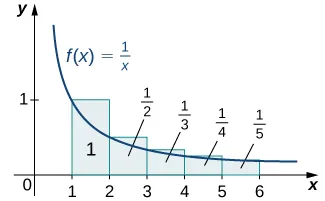
\includegraphics[scale=0.5]{./figures/mane9.png}
    \end{center}
    \bigbreak \noindent 
    Now consider the series $\sum_{n=1}^{\infty} \frac{1}{n^2}$. We show how an integral can be used to prove that this series converges. In Figure 5.13, we sketch a sequence of rectangles with areas $1, \frac{1}{2^2}, \frac{1}{3^2}, \ldots$ along with the function $f(x) = \frac{1}{x^2}$. From the graph, we see that
    \bigbreak \noindent 
    \begin{align*}
        \sum_{n=1}^{k} \frac{1}{n^2} = 1 + \frac{1}{2^2} + \frac{1}{3^2} + \cdots + \frac{1}{k^2} < 1 + \int_{1}^{k} \frac{1}{x^2} \, dx.
    .\end{align*}
    Therefore, for each $k$, the $k$th partial sum $S_k$ satisfies
    \[ S_k = \sum_{n=1}^{k} \frac{1}{n^2} < 1 + \int_{1}^{k} \frac{1}{x^2} \, dx = 1 - \frac{1}{x} \Bigg|_{1}^{k} = 1 - \frac{1}{k} + 1 = 2 - \frac{1}{k} < 2. \]
    We conclude that the sequence of partial sums $\{S_k\}$ is bounded. We also see that $\{S_k\}$ is an increasing sequence:
    \[ S_k = S_{k-1} + \frac{1}{k^2} \quad \text{for} \quad k \geq 2. \]
    Since $\{S_k\}$ is increasing and bounded, by the Monotone Convergence Theorem, it converges. Therefore, the series $\sum_{n=1}^{\infty} \frac{1}{n^2}$ converges.
    \bigbreak \noindent 
    \begin{center}
        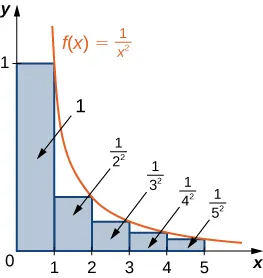
\includegraphics[scale=0.5]{./figures/mane10.png}
    \end{center}
    \bigbreak \noindent 
    We can extend this idea to prove convergence or divergence for many different series. Suppose $\sum_{n=1}^{\infty} a_n$ is a series with positive terms $a_n$ such that there exists a continuous, positive, decreasing function $f$ where $f(n) = a_n$ for all positive integers. Then, as in Figure 5.14(a), for any integer $k$, the $k$th partial sum $S_k$ satisfies
    \[
    S_k = a_1 + a_2 + a_3 + \cdots + a_k < a_1 + \int_{1}^{k} f(x) \, dx < a_1 + \int_{1}^{\infty} f(x) \, dx.
    \]
    Therefore, if $\int_{1}^{\infty} f(x) \, dx$ converges, then the sequence of partial sums $\{S_k\}$ is bounded. Since $\{S_k\}$ is an increasing sequence, if it is also a bounded sequence, then by the Monotone Convergence Theorem, it converges. We conclude that if $\int_{1}^{\infty} f(x) \, dx$ converges, then the series $\sum_{n=1}^{\infty} a_n$ also converges. On the other hand, from Figure 5.14(b), for any integer $k$, the $k$th partial sum $S_k$ satisfies
    \[
    S_k = a_1 + a_2 + a_3 + \cdots + a_k > \int_{1}^{k+1} f(x) \, dx.
    \]
    If $\lim_{k \to \infty} \int_{1}^{k+1} f(x) \, dx = \infty$, then $\{S_k\}$ is an unbounded sequence and therefore diverges. As a result, the series $\sum_{n=1}^{\infty} a_n$ also diverges. We conclude that if $\int_{1}^{\infty} f(x) \, dx$ diverges, then $\sum_{n=1}^{\infty} a_n$ diverges.
    \bigbreak \noindent 

    \begin{thrm}[Integral Test]
        Suppose  $\summation{\infty}{n=1}\ a_{n}\  $ is a series with positive terms  $a_{n}$ Suppose there exists a function  $f $
  and a positive integer  $N$ 
  such that the following three conditions are satisfied:
        \begin{enumerate}
            \item \( f \) continuous
            \item \( f \) positive and decreasing
            \item \( f(n) = a_n \) for all integers \( n \geq N \),
        \end{enumerate}
        \begin{align*}
            \text{Then the series} \sum_{n=1}^{\infty} a_n \text{ and the improper integral} \int_{N}^{\infty} f(x) \, dx \text{ either both converge or both diverge.}
        .\end{align*}

    \end{thrm}
    \bigbreak \noindent 
    Although convergence of \( \int_{N}^{\infty} f(x) \, dx \)
    implies convergence of the related series \( \sum_{n=1}^{\infty} a_n \),
    it does not imply that the value of the integral and the series are the same. They may be different, and often are. For example,
    \[
    \sum_{n=1}^{\infty} \left(\frac{1}{e}\right)^n = \frac{1}{e} + \left(\frac{1}{e}\right)^2 + \left(\frac{1}{e}\right)^3 + \cdots
    \]
    is a geometric series with initial term \( a=\frac{1}{e} \)
    and ratio \( r=\frac{1}{e} \),
    which converges to
    \[
    \frac{\frac{1}{e}}{1-\left(\frac{1}{e}\right)} = \frac{1}{e} \cdot \frac{e-1}{e} = \frac{1}{e-1}.
    \]
    However, the related integral \( \int_{1}^{\infty} \left(\frac{1}{e}\right)^x \, dx \)
    satisfies
    \[
    \int_{1}^{\infty} \left(\frac{1}{e}\right)^x \, dx = \int_{1}^{\infty} e^{-x} \, dx = \lim_{b \to \infty} \int_{1}^{b} e^{-x} \, dx = \lim_{b \to \infty} \left[-e^{-x}\right]_{1}^{b} = \lim_{b \to \infty} \left[-e^{-b} + e^{-1}\right] = \frac{1}{e}.
    \]


    \pagebreak 
    \phantomsection
    \addcontentsline{toc}{subsection}{The p-series}
    \subsection*{The p-series}
    \bigbreak \noindent 
    The harmonic series \( \sum_{n=1}^{\infty} \frac{1}{n} \)
    and the series \( \sum_{n=1}^{\infty} \frac{1}{n^2} \)
    are both examples of a type of series called a \( p \)-series.

    \bigbreak \noindent 
    \begin{definition}
       $\forall p \in \mathbb{R}$, the series 
       \begin{align*}
           \summation{\infty}{n=1}\ \frac{1}{n^{P}}\ 
       .\end{align*}
       Is called a \textbf{p-series}
    \end{definition}

    \bigbreak \noindent 
    We know the \( p \)-series converges if \( p=2 \) and diverges if \( p=1 \).
What about other values of \( p \)?
In general, it is difficult, if not impossible, to compute the exact value of most \( p \)-series. However, we can use the tests presented thus far to prove whether a \( p \)-series converges or diverges.
\bigbreak \noindent 
If \( p<0 \), then \( \frac{1}{n^p} \to \infty \), and if \( p=0 \), then \( \frac{1}{n^p} \to 1 \).
Therefore, by the divergence test,
\begin{align}
\sum_{n=1}^{\infty} \frac{1}{n^p} \text{ diverges if } p \leq 0.
\end{align}
If \( p>0 \), then \( f(x) = \frac{1}{x^p} \) is a positive, continuous, decreasing function. Therefore, for \( p>0 \), we use the integral test, comparing
\begin{align}
\sum_{n=1}^{\infty} \frac{1}{n^p} \quad \text{and} \quad \int_{1}^{\infty} \frac{1}{x^p} \, dx.
\end{align}
We have already considered the case when \( p=1 \).
Here we consider the case when \( p>0, p \neq 1 \).
For this case,
\begin{align}
\int_{1}^{\infty} \frac{1}{x^p} \, dx &= \lim_{b \to \infty} \int_{1}^{b} \frac{1}{x^p} \, dx \\
&= \lim_{b \to \infty} \left[ \frac{1}{1-p} x^{1-p} \right]_{1}^{b} \\
&= \lim_{b \to \infty} \left[ \frac{1}{1-p} \left( b^{1-p} - 1 \right) \right].
\end{align}
Because
\begin{align}
b^{1-p} \to 0 &\text{ if } p>1 \text{ and} \\
b^{1-p} \to \infty &\text{ if } p<1,
\end{align}
we conclude that
\begin{align}
\int_{1}^{\infty} \frac{1}{x^p} \, dx =
\begin{cases}
\frac{1}{p-1} & \text{if } p>1 \\
\infty & \text{if } p \leq 1.
\end{cases}
\end{align}
Therefore, \( \sum_{n=1}^{\infty} \frac{1}{n^p} \)
converges if \( p>1 \)
and diverges if \( 0<p<1 \).
\bigbreak \noindent 

In summary,
\begin{align}
\sum_{n=1}^{\infty} \frac{1}{n^p} \begin{cases}
\text{converges if } p>1 \\
\text{diverges if } p \leq 1.
\end{cases}
\end{align}

    \pagebreak 
    \phantomsection
    \addcontentsline{toc}{subsection}{Estimating the Value of a Series}
    \subsection*{Estimating the Value of a Series}
    \bigbreak \noindent 
    Suppose we know that a series \( \sum_{n=1}^{\infty} a_n \)
converges and we want to estimate the sum of that series. Certainly, we can approximate that sum using any finite sum \( \sum_{n=1}^{N} a_n \)
where \( N \)
is any positive integer. The question we address here is, for a convergent series \( \sum_{n=1}^{\infty} a_n \),
how good is the approximation \( \sum_{n=1}^{N} a_n \)?
More specifically, if we let
\[ R_N = \sum_{n=1}^{\infty} a_n - \sum_{n=1}^{N} a_n \]
be the remainder when the sum of an infinite series is approximated by the \( N \)th
partial sum, how large is \( R_N \)?
For some types of series, we are able to use the ideas from the integral test to estimate \( R_N \).
    
    \bigbreak \noindent 
    \begin{thrm}[Remainder Estimate from the Integral Test]
        Suppose \( \sum_{n=1}^{\infty} a_n \)
        is a convergent series with positive terms. Suppose there exists a function \( f \)
        satisfying the following three conditions:
        \begin{enumerate}
            \item \( f \) is continuous,
            \item \( f \) is decreasing, and
            \item \( f(n) = a_n \) for all integers \( n \geq 1 \).
        \end{enumerate}
        Let \( S_N \) be the \( N \)th partial sum of \( \sum_{n=1}^{\infty} a_n \).
        For all positive integers \( N \),
        \[
        S_N + \int_{N+1}^{\infty} f(x) \, dx < \sum_{n=1}^{\infty} a_n < S_N + \int_{N}^{\infty} f(x) \, dx.
        \]
        In other words, the remainder \( R_N = \sum_{n=1}^{\infty} a_n - S_N = \sum_{n=N+1}^{\infty} a_n \)
        satisfies the following estimate:
        \[
        \int_{N+1}^{\infty} f(x) \, dx < R_N < \int_{N}^{\infty} f(x) \, dx.
        \]
        This is known as the remainder estimate 
    \end{thrm}
    \bigbreak \noindent 
    We illustrate the Remainder Estimate from the Integral Test in Figure 5.15. In particular, by representing the remainder \( R_N = a_{N+1} + a_{N+2} + a_{N+3} + \cdots \)
    as the sum of areas of rectangles, we see that the area of those rectangles is bounded above by \( \int_{N}^{\infty} f(x) \, dx \)
    and bounded below by \( \int_{N+1}^{\infty} f(x) \, dx \).
    In other words,
    \[
    R_N = a_{N+1} + a_{N+2} + a_{N+3} + \cdots > \int_{N+1}^{\infty} f(x) \, dx
    \]
    and
    \[
    R_N = a_{N+1} + a_{N+2} + a_{N+3} + \cdots < \int_{N}^{\infty} f(x) \, dx.
    \]
    We conclude that
    \[
    \int_{N+1}^{\infty} f(x) \, dx < R_N < \int_{N}^{\infty} f(x) \, dx.
    \]
    Since
    \[
    \sum_{n=1}^{\infty} a_n = S_N + R_N,
    \]
    where \( S_N \)
    is the \( N \)th partial sum, we conclude that
    \[
    S_N + \int_{N+1}^{\infty} f(x) \, dx < \sum_{n=1}^{\infty} a_n < S_N + \int_{N}^{\infty} f(x) \, dx.
    \]

    \pagebreak \bigbreak \noindent 
    \begin{center}
        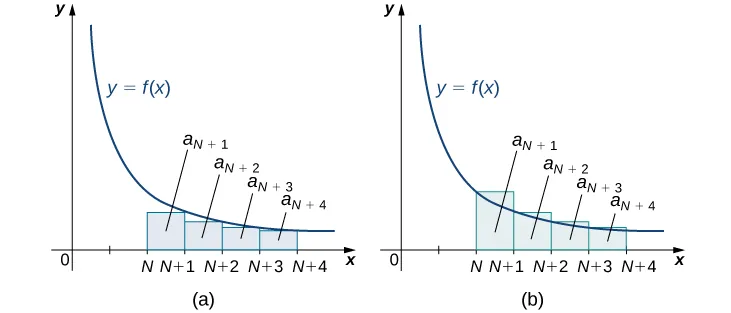
\includegraphics[scale=0.5]{./figures/mane11.png}
    \end{center}
    \bigbreak \noindent 
    \begin{eg}[Estimating the Value of a Series]
        Consider the series 
        \begin{align*}
            \summation{\infty}{n=1}\ \frac{1}{n^{3}}\ 
        .\end{align*}
        \begin{enumerate}[label=(\alph*)]
            \item Calculate $S_{10} = \summation{10}{n=1}\ \frac{1}{n^{3}}\ $
            \item Determine the least value of  $N$ necessary such that  $S_{N} $ will estimate  $\summation{\infty}{n=1}\ \frac{1}{n^{3}}\  $ to within 0.001
        \end{enumerate}
    \end{eg}
    \bigbreak \noindent 
    \textbf{Solution.} Computing $S_{10}$, we get:
    \begin{align*}
        S_{10} \approx 1.19753
    .\end{align*}
    \bigbreak \noindent 
    By the remainder estimate, we know
    \begin{align*}
        R_{N} < \int_{N}^{\infty}\ \frac{1}{x^{3}}\ dx
    .\end{align*}
    \bigbreak \noindent 
    We have:
    \[
        \int_{10}^{\infty} \frac{1}{x^3} \, dx = \lim_{b \to \infty} \int_{10}^{b} \frac{1}{x^3} \, dx = \lim_{b \to \infty} \left[ -\frac{1}{2x^2} \right]_{10}^{b} = \lim_{b \to \infty} \left[ -\frac{1}{2b^2} + \frac{1}{2N^{2}} \right] = \frac{1}{2N^{2}}.
    \]
    \bigbreak \noindent 
    Thus, the error is $R_{10}  < \frac{1}{2(10)^{2}} = 0.005$
    \bigbreak \noindent 
    Since we have showed that $R_{N} < \frac{1}{2N^{2}}$, the remainder $R_{N} < 0.001$ as long as $\frac{1}{2N^{2}} < 0.001 $. That is, we need $2N^{2} > 1000$. Solving for $N$ we get $22.36$. Therefore, we should use $N=23$

    \pagebreak 
    \phantomsection
    \addcontentsline{toc}{section}{5.4 Comparison Tests}
    \section*{5.4 Comparison Tests}
    \bigbreak \noindent 
    In the preceding two sections, we discussed two large classes of series: geometric series and p-series. We know exactly when these series converge and when they diverge. Here we show how to use the convergence or divergence of these series to prove convergence or divergence for other series, using a method called the comparison test.
    For example, consider the series
    \[
    \sum_{n=1}^{\infty} \frac{1}{n^2+1}.
    \]
    This series looks similar to the convergent series
    \[
    \sum_{n=1}^{\infty} \frac{1}{n^2}.
    \]
    Since the terms in each of the series are positive, the sequence of partial sums for each series is monotone increasing. Furthermore, since
    \[
    0 < \frac{1}{n^2+1} < \frac{1}{n^2}
    \]
    for all positive integers \( n \), the \( k \)th partial sum \( S_k \) of \( \sum_{n=1}^{\infty} \frac{1}{n^2+1} \) satisfies
    \[
    S_k = \sum_{n=1}^{k} \frac{1}{n^2+1} < \sum_{n=1}^{k} \frac{1}{n^2} < \sum_{n=1}^{\infty} \frac{1}{n^2}.
    \]
    \bigbreak \noindent 
    Since the series on the right converges, the sequence \(\{S_k\}\) is bounded above. We conclude that \(\{S_k\}\) is a monotone increasing sequence that is bounded above. Therefore, by the Monotone Convergence Theorem, \(\{S_k\}\) converges, and thus
    \begin{align}
    \sum_{n=1}^{\infty} \frac{1}{n^2+1}
    \end{align}
    converges.

    \bigbreak \noindent 
    \begin{thrm}[Comparison Test for series]
        \begin{enumerate}
            \item Suppose there exists an integer \( N \) such that \( 0 \leq a_n \leq b_n \) for all \( n \geq N \). If \( \sum_{n=1}^{\infty} b_n \) converges, then \( \sum_{n=1}^{\infty} a_n \) converges. 
            \item  Suppose there exists an integer \( N \) such that \( a_n \geq b_n \geq 0 \) for all \( n \geq N \). If \( \sum_{n=1}^{\infty} b_n \) diverges, then \( \sum_{n=1}^{\infty} a_n \) diverges.
        \end{enumerate}
    \end{thrm}
    \bigbreak \noindent 
    
    \pagebreak \bigbreak \noindent 
       \begin{eg}[Using the comparison test for series]
        Use theorem 11 to show the convergence or divergence of the series
        \begin{align*}
            \summation{\infty}{n=1}\ \frac{1}{n^{3}+3n+1}\ 
        .\end{align*}
    \end{eg}
    \bigbreak \noindent 
    \textbf{Solution.} We can compare this series to  $\summation{\infty}{n=1}\ \frac{1}{n^{3}}\ $. Since this new series is a $p$-series with $p >1$,  we know it will converge. Furthermore, since 
    \begin{align*}
        \frac{1}{n^{3} + 3n + 1} < \frac{1}{n^{3}}
    .\end{align*}
    $\forall\ n \in \mathbb{Z^{+}}$, we can canclude that the series $\summation{\infty}{n=1}\ \frac{1}{n^{3}+3n+1}\ $ converges

    \bigbreak \noindent 
   \begin{eg}[Using the comparison test for series]
        Use theorem 11 to show the convergence or divergence of the series
        \begin{align*}
            \summation{\infty}{n=2}\ \frac{1}{\ln{n}}\ 
        .\end{align*}
    \end{eg}
    \bigbreak \noindent 
    \textbf{Solution.} We can compare this series to $\summation{\infty}{n=2}\ \frac{1}{n}\ $. Since
    \begin{align*}
        \frac{1}{\ln{n}} > \frac{1}{n}
    .\end{align*}
    \bigbreak \noindent 
    $\forall\ n \geq 2, n \in \mathbb{Z^{+}}$, and since $\summation{\infty}{n=2}\ \frac{1}{n}\ $ diverges, we can conclude that the series $\summation{\infty}{n=2}\ \frac{1}{\ln{n}}\  $ also diverges

    \bigbreak \noindent 
    \phantomsection
    \addcontentsline{toc}{subsection}{Limit Comparison Test}
    \subsection*{Limit Comparison Test}
    \bigbreak \noindent 
    The comparison test works nicely if we can find a comparable series satisfying the hypothesis of the test. However, sometimes finding an appropriate series can be difficult. Consider the series
    \[
    \sum_{n=2}^{\infty} \frac{1}{n^2 - 1}.
    \]
    It is natural to compare this series with the convergent series
    \[
    \sum_{n=2}^{\infty} \frac{1}{n^2}.
    \]
    However, this series does not satisfy the hypothesis necessary to use the comparison test because
    \[
    \frac{1}{n^2 - 1} > \frac{1}{n^2}
    \]
    for all integers \( n \geq 2 \). Although we could look for a different series with which to compare \( \sum_{n=2}^{\infty} \frac{1}{n^2 - 1} \), instead we show how we can use the limit comparison test to compare
    \[
    \sum_{n=2}^{\infty} \frac{1}{n^2 - 1} \quad \text{and} \quad \sum_{n=2}^{\infty} \frac{1}{n^2}.
    \]
    Let us examine the idea behind the limit comparison test. Consider two series \( \sum_{n=1}^{\infty} a_n \) and \( \sum_{n=1}^{\infty} b_n \) with positive terms \( a_n \) and \( b_n \) and evaluate
    \[
    \lim_{n \to \infty} \frac{a_n}{b_n}.
    \]
    If
    \[
    \lim_{n \to \infty} \frac{a_n}{b_n} = L \neq 0,
    \]
    then, for \( n \) sufficiently large, \( a_n \approx Lb_n \). Therefore, either both series converge or both series diverge. For the series \( \sum_{n=2}^{\infty} \frac{1}{n^2 - 1} \) and \( \sum_{n=2}^{\infty} \frac{1}{n^2} \), we see that
    \[
    \lim_{n \to \infty} \frac{1/(n^2 - 1)}{1/n^2} = \lim_{n \to \infty} \frac{n^2}{n^2 - 1} = 1.
    \]
    Since \( \sum_{n=2}^{\infty} \frac{1}{n^2} \) converges, we conclude that
    \[
    \sum_{n=2}^{\infty} \frac{1}{n^2 - 1}
    \]
    converges.
    \bigbreak \noindent 
    The limit comparison test can be used in two other cases. Suppose
    \[
    \lim_{n \to \infty} \frac{a_n}{b_n} = 0.
    \]
    In this case, \( \{ a_n/b_n \} \) is a bounded sequence. As a result, there exists a constant \( M \) such that \( a_n \leq M b_n \). Therefore, if \( \sum_{n=1}^{\infty} b_n \) converges, then \( \sum_{n=1}^{\infty} a_n \) converges. On the other hand, suppose
    \[
    \lim_{n \to \infty} \frac{a_n}{b_n} = \infty.
    \]
    In this case, \( \{ a_n/b_n \} \) is an unbounded sequence. Therefore, for every constant \( M \) there exists an integer \( N \) such that \( a_n \geq M b_n \) for all \( n \geq N \). Therefore, if \( \sum_{n=1}^{\infty} b_n \) diverges, then \( \sum_{n=1}^{\infty} a_n \) diverges as well.


    \bigbreak \noindent 
    \begin{thrm}[Limit Comparison Test]
     Let \( a_n, b_n \geq 0 \) for all \( n \geq 1 \).
        \begin{itemize}
          \item If \( \lim_{n \to \infty} \frac{a_n}{b_n} = L \neq 0 \), then \( \sum_{n=1}^{\infty} a_n \) and \( \sum_{n=1}^{\infty} b_n \) both converge or both diverge.
          \item If \( \lim_{n \to \infty} \frac{a_n}{b_n} = 0 \) and \( \sum_{n=1}^{\infty} b_n \) converges, then \( \sum_{n=1}^{\infty} a_n \) converges.
          \item If \( \lim_{n \to \infty} \frac{a_n}{b_n} = \infty \) and \( \sum_{n=1}^{\infty} b_n \) diverges, then \( \sum_{n=1}^{\infty} a_n \) diverges.
        \end{itemize}
    \end{thrm}
    \bigbreak \noindent 
    Note that if $\frac{a_n}{b_n} \to 0$ and $\sum_{n=1}^{\infty} b_n$ diverges, the limit comparison test gives no information. Similarly, if $\frac{a_n}{b_n} \to \infty$ and $\sum_{n=1}^{\infty} b_n$ converges, the test also provides no information. For example, consider the two series $\sum_{n=1}^{\infty} \frac{1}{\sqrt{n}}$ and $\sum_{n=1}^{\infty} \frac{1}{n^2}$. These series are both $p$-series with $p=\frac{1}{2}$ and $p=2$, respectively. Since $p=\frac{1}{2} < 1$, the series $\sum_{n=1}^{\infty} \frac{1}{\sqrt{n}}$ diverges. On the other hand, since $p=2 > 1$, the series $\sum_{n=1}^{\infty} \frac{1}{n^2}$ converges. However, suppose we attempted to apply the limit comparison test, using the convergent $p$-series $\sum_{n=1}^{\infty} \frac{1}{n^3}$ as our comparison series. First, we see that
    \bigbreak \noindent 
    \[
    \frac{\frac{1}{\sqrt{n}}}{\frac{1}{n^3}} = \frac{n^3}{\sqrt{n}} = n^{\frac{5}{2}} \to \infty \text{ as } n \to \infty.
    \]
    Similarly, we see that
    \[
    \frac{\frac{1}{n^2}}{\frac{1}{n^3}} = n \to \infty \text{ as } n \to \infty.
    \]
    Therefore, if $\frac{a_n}{b_n} \to \infty$ when $\sum_{n=1}^{\infty} b_n$ converges, we do not gain any information on the convergence or divergence of $\sum_{n=1}^{\infty} a_n$.

   \pagebreak \bigbreak \noindent  
   \begin{eg}
      use the limit comparison test to determine whether the series converges or diverges. If the test does not apply, say so. 
      \begin{align*}
          \summation{\infty}{n=1}\ \frac{1}{\sqrt{n} + 1}\ 
      .\end{align*}
   \end{eg}
   \bigbreak \noindent 
   \textbf{Solution.} We compare to $\frac{1}{\sqrt{n}}$, by the p-series  we know that $\summation{\infty}{n=1}\ \frac{1}{\sqrt{n}}\  $ Diverges, since $\frac{1}{\sqrt{n} + 1} < \frac{1}{\sqrt{n}}$. We must use the limit comparison test. Thus, 
   \begin{align*}
       &\lim\limits_{n \to \infty}{\frac{\frac{1}{\sqrt{n+1}}}{\frac{1}{\sqrt{n}}}} \\
       &=\lim\limits_{n \to \infty}{\frac{\sqrt{n}}{\sqrt{n+1}}} \\
       &= 1
   .\end{align*}
   \bigbreak \noindent 
   Since $\lim\limits_{n \to \infty}{\frac{a_{n}}{b_{n}}} = L \ne 0$, then since $b_{n} $ diverges, so does $a_{n} $

   \pagebreak 
   \phantomsection
   \addcontentsline{toc}{section}{5.5 Alternating Series}
   \section*{5.5 Alternating Series}

   \bigbreak \noindent 
   \phantomsection
   \addcontentsline{toc}{subsection}{The Alternating Series Test}
   \subsection*{The Alternating Series Test}
   \bigbreak \noindent 
   A series whose terms alternate between positive and negative values is an alternating series. For example, the series
   \begin{align*}
        \sum_{n=1}^{\infty} \left(-\frac{1}{2}\right)^n = -\frac{1}{2} + \frac{1}{4} - \frac{1}{8} + \frac{1}{16} - \cdots
   .\end{align*}
   \bigbreak \noindent 
   and
   \begin{align*}
       \sum_{n=1}^{\infty} \frac{(-1)^{n+1}}{n}  = 1 - \frac{1}{2} + \frac{1}{3} - \frac{1}{4} + \cdots
   .\end{align*}
   are both alternating series.

   \bigbreak \noindent 
   \begin{definition}
      Any series whose terms alternate between positive and negative values is called an alternating series. An alternating series can be written in the form 
      \begin{align*}
          \sum_{n=1}^{\infty} (-1)^{n+1} b_n = b_1 - b_2 + b_3 - b_4 + \cdots
      .\end{align*}
      or
      \begin{align*}
          \sum_{n=1}^{\infty} (-1)^n b_n = -b_1 + b_2 - b_3 + b_4 - \cdots
      .\end{align*}
      Where  $b_n > 0$  for all positive integers $n$.

   \end{definition}
   \bigbreak \noindent 
   \begin{thrm}[Alternating Series Test]
       An alternating series of the form
        \[
        \sum_{n=1}^{\infty} (-1)^{n+1} b_n \quad \text{or} \quad \sum_{n=1}^{\infty} (-1)^n b_n
        \]
        converges if
        \begin{itemize}
            
            \item $0 < b_{n+1} \leq b_n\ \forall\ n \geq 1$
            \item $\lim_{n \to \infty} b_n = 0.$
    \end{itemize}

    This is known as the alternating series test.
   \end{thrm}

   \pagebreak \bigbreak \noindent 
   \begin{eg}[Using the Leibniz criterion (AST)]
      determine whether the series converges or diverges. 
      \begin{align*}
          \summation{\infty}{n=1}\ \frac{(-1)^{n+1}}{n^{2}}\ 
      .\end{align*}
   \end{eg}
   \bigbreak \noindent 
    \textbf{Solution.} To apply the Leibniz criterion (AST), we consider the sequence \( b_n = \frac{1}{n^2} \), which are the absolute values of the terms of the given series. We need to show that this sequence is decreasing. For all \( n \geq 1 \),
    \begin{align*}
    b_{n} &= \frac{1}{n^2}, \\
    b_{n+1} &= \frac{1}{(n+1)^2}.
    \end{align*}
    We see that \( (n+1)^2 > n^2 \) for all \( n \geq 1 \), which implies that \( b_{n+1} < b_n \). Therefore, the sequence \( \{b_n\} \) is monotonically decreasing.
    \bigbreak \noindent 
    Additionally, we need to show that \( \lim_{n \to \infty} b_n = 0 \):
    \begin{align*}
        \lim_{n \to \infty} b_n = \lim_{n \to \infty} \frac{1}{n^2} = 0.
    \end{align*}
    Since both conditions of the Leibniz criterion are satisfied, the series \( \sum_{n=1}^{\infty} \frac{(-1)^{n+1}}{n^{2}} \) converges.

    \bigbreak \noindent 
    Since
    \begin{align*}
        \frac{1}{(n+1)^{2}} < \frac{1}{n^{2}} \quad \text{and } \frac{1}{n^{2}} \to 0
    .\end{align*}
    The series converges

   \bigbreak \noindent 
  \begin{eg}[Using the Leibniz criterion (AST)]
      determine whether the series converges or diverges. 
      \begin{align*}
          \summation{\infty}{n=1}\ \frac{n(-1)^{n+1}}{n+1}\ 
      .\end{align*}
   \end{eg}
   \bigbreak \noindent 
   \textbf{Solution.} Since $\frac{n}{n+1} \nrightarrow 0$ as $n \rightarrow \infty$.  we cannot apply the alternating series test. Instead, we use the nth term test for divergence. Since
   \begin{align*}
       \lim\limits_{n \to \infty}{\frac{(-1)^{n+1}n}{n+1}} \ne 0 
   .\end{align*}
   \bigbreak \noindent 
   The series diverges

   \pagebreak
   \phantomsection
   \addcontentsline{toc}{subsection}{Remainder of an Alternating Series}
   \subsection*{Remainder of an Alternating Series}
   \bigbreak \noindent 
    It is difficult to explicitly calculate the sum of most alternating series, so typically the sum is approximated by using a partial sum. When doing so, we are interested in the amount of error in our approximation. Consider an alternating series
    \begin{align*}
        \summation{\infty}{n=1}\ (-1)^{n+1}b_{n}\ 
    .\end{align*}
    \bigbreak \noindent 
    satisfying the hypotheses of the alternating series test. Let \( S \) denote the sum of this series and \( \{S_k\} \) be the corresponding sequence of partial sums. From Figure 5.18, we see that for any integer \( N \geq 1 \), the remainder \( R_N \) satisfies
    \begin{align*}
        \lvert R_N \rvert = \lvert S - S_N \rvert \leq \lvert S_{N+1} - S_N \rvert = b_{n+1} 
    .\end{align*}
    \bigbreak \noindent 
    This tells us that if we stop at the $N^{th}$ term, the error we are making is at most the size of the next term we did not include.
    \bigbreak \noindent 
    \begin{thrm}[Remainders in Alternating Series]
        Consider an alternating series of the form
\[
\sum_{n=1}^{\infty} (-1)^{n+1} b_n \quad \text{or} \quad \sum_{n=1}^{\infty} (-1)^n b_n,
\]
that satisfies the hypotheses of the alternating series test. Let \( S \) denote the sum of the series and \( S_N \) denote the \( N \)-th partial sum. For any integer \( N \geq 1 \), the remainder \( R_N = S - S_N \) satisfies
\[
\lvert R_N \rvert \leq b_{N+1}.
\]

    \end{thrm}

    \bigbreak \noindent 
    \begin{eg}[Remainder estimate in alternating series]
        Consider the alternating series
        \begin{align*}
            \summation{\infty}{n=1}\ \frac{(-1)^{n+1}}{n^{2}}\ 
        .\end{align*}
        \bigbreak \noindent 
        Use the remainder estimate to determine a bound on the error  $R_{10}$ if we approximate the sum of the series by the partial sum  $S_{10}$
    \end{eg}
    \bigbreak \noindent 
    \textbf{Solution.} 
    \begin{align*}
        R_{10} \leq b_{11} = \frac{1}{11^{2}} \approx 0.008265
    .\end{align*}

    \pagebreak 
    \phantomsection
    \addcontentsline{toc}{subsection}{Absolute and Conditional Convergence}
    \subsection*{Absolute and Conditional Convergence}
    \bigbreak \noindent 
    Consider a series \(\sum_{n=1}^{\infty} a_n\) and the related series \(\sum_{n=1}^{\infty} |a_n|\). Here we discuss possibilities for the relationship between the convergence of these two series. For example, consider the alternating harmonic series \(\sum_{n=1}^{\infty} (-1)^{n+1}/n\). The series whose terms are the absolute value of these terms is the harmonic series, since \(\sum_{n=1}^{\infty} |(-1)^{n+1}/n| = \sum_{n=1}^{\infty} 1/n\). Since the alternating harmonic series converges, but the harmonic series diverges, we say the alternating harmonic series exhibits conditional convergence.
    \bigbreak \noindent 
    By comparison, consider the series \(\sum_{n=1}^{\infty} (-1)^{n+1}/n^2\). The series whose terms are the absolute values of the terms of this series is the series \(\sum_{n=1}^{\infty} 1/n^2\). Since both of these series converge, we say the series \(\sum_{n=1}^{\infty} (-1)^{n+1}/n^2\) exhibits absolute convergence.
    \bigbreak \noindent 
    \begin{definition}
        \begin{enumerate}[label=\roman*.]
            \item A series \(\sum_{n=1}^{\infty} a_n\) exhibits absolute convergence if \(\sum_{n=1}^{\infty} |a_n|\) converges. (converges absolutely)
            \item A series \(\sum_{n=1}^{\infty} a_n\) exhibits conditional convergence if \(\sum_{n=1}^{\infty} a_n\) converges but \(\sum_{n=1}^{\infty} |a_n|\) diverges.
            \item If $\summation{\infty}{n=1}\ \lvert a_{n} \rvert\ $ converges then $\summation{\infty}{n=1}\ a_{n}\ $ converges
        \end{enumerate}
    \end{definition}

    \pagebreak
    \phantomsection
    \addcontentsline{toc}{section}{5.6 Ratio and Root Tests}
    \section*{5.6 Ratio and Root Tests}
    \bigbreak \noindent 
    Consider a series \(\sum_{n=1}^{\infty} a_n\).
    From our earlier discussion and examples, we know that \(\lim_{n \to \infty} a_n = 0\)
    is not a sufficient condition for the series to converge. Not only do we need \(a_n \to 0\),
    but we need \(a_n \to 0\) quickly enough. For example, consider the series \(\sum_{n=1}^{\infty} \frac{1}{n}\)
    and the series \(\sum_{n=1}^{\infty} \frac{1}{n^2}\).
    We know that \(\frac{1}{n} \to 0\)
    and \(\frac{1}{n^2} \to 0\).
    However, only the series \(\sum_{n=1}^{\infty} \frac{1}{n^2}\)
    converges. The series \(\sum_{n=1}^{\infty} \frac{1}{n}\)
    diverges because the terms in the sequence \(\{ \frac{1}{n} \}\)
    do not approach zero fast enough as \(n \to \infty\).
    Here we introduce the ratio test, which provides a way of measuring how fast the terms of a series approach zero.

    \bigbreak \noindent 
    \begin{thrm}[Ratio Test]
       Let \(\sum_{n=1}^{\infty} a_n\) be a series with nonzero terms. Let
        \[
        \rho = \lim_{n \to \infty} \left| \frac{a_{n+1}}{a_n} \right|.
        \]
        Then:
        \begin{enumerate}[label=\roman*.]
            \item If \(0 \leq \rho < 1\), then \(\sum_{n=1}^{\infty} a_n\) converges absolutely.
            \item If \(\rho > 1\) or \(\rho = \infty\), then \(\sum_{n=1}^{\infty} a_n\) diverges.
            \item If \(\rho = 1\), the test does not provide any information.
        \end{enumerate}
    \end{thrm}

    \bigbreak \noindent 
    \phantomsection
    \addcontentsline{toc}{subsection}{Root Test}
    \subsection*{Root Test}
    \bigbreak \noindent 
    The approach of the root test is similar to that of the ratio test. Consider a series \(\sum_{n=1}^{\infty} a_n\) such that \(\lim_{n \to \infty} \sqrt[n]{|a_n|} = \rho\) for some real number \(\rho\). Then for \(N\) sufficiently large, \(|a_N| \approx \rho^N\). Therefore, we can approximate \(\sum_{n=N}^{\infty} |a_n|\) by writing
    \[
    |a_N| + |a_{N+1}| + |a_{N+2}| + \cdots \approx \rho^N + \rho^{N+1} + \rho^{N+2} + \cdots.
    \]
    The expression on the right-hand side is a geometric series. As in the ratio test, the series \(\sum_{n=1}^{\infty} a_n\) converges absolutely if \(0 \leq \rho < 1\) and the series diverges if \(\rho \geq 1\). If \(\rho = 1\), the test does not provide any information. For example, for any \(p\)-series, \(\sum_{n=1}^{\infty} \frac{1}{n^p}\), we see that
    \[
    \rho = \lim_{n \to \infty} \sqrt[n]{\left|\frac{1}{n^p}\right|} = \lim_{n \to \infty} \frac{1}{n^{p/n}}.
    \]
    To evaluate this limit, we use the natural logarithm function. Doing so, we see that
    \[
    \ln(\rho) = \ln\left(\lim_{n \to \infty} \frac{1}{n^{p/n}}\right) = \lim_{n \to \infty} \ln\left(\frac{1}{n}\right)^{p/n} = \lim_{n \to \infty} \frac{p \ln(1/n)}{n}.
    \]
    Using L'Hôpital's rule, it follows that \(\ln(\rho) = 0\), and therefore \(\rho = 1\) for all \(p\). However, we know that the \(p\)-series only converges if \(p > 1\) and diverges if \(p \leq 1\).

    \pagebreak \bigbreak \noindent 
    \begin{thrm}[Root Test]
        Consider the series \(\sum_{n=1}^{\infty} a_n\). Let
        \[
        \rho = \lim_{n \to \infty} \sqrt[n]{|a_n|}.
        \]
        \begin{enumerate}[label=\roman*.]
            \item If \(0 \leq \rho < 1\), then \(\sum_{n=1}^{\infty} a_n\) converges absolutely. 
            \item If \(\rho > 1\) or \(\rho = \infty\), then \(\sum_{n=1}^{\infty} a_n\) diverges. 
            \item If \(\rho = 1\), the test does not provide any information.
        \end{enumerate}
    \end{thrm}
    \bigbreak \noindent 
    The root test is useful for series whose terms involve exponentials. In particular, for a series whose terms \(a_n\) satisfy \(|a_n| = b_n^n\), then \(\sqrt[n]{|a_n|} = b_n\) and we need only evaluate \(\lim_{n \to \infty} b_n\).

    

        

    

    
    

   


   
   
   

   

    
 




    


    

        



\end{document}
